% app2.tex (file to switch to appendix mode)

\invisiblechapter{\bassPiece}

\vspace{3.8cm}

\begin{center}

\textsc{for solo contrabass}

\vspace{2.8cm}

\HRule{0.5pt}

\LARGE \textbf{\uppercase{\bassPiece}}

\HRule{2pt}

\vspace{1.8cm}

\normalsize \today

\vspace{3.8cm}

Rhys Gray

\end{center}
\newpage

\section*{Program Notes}
Inspired by the eponymous short story by Ray Bradbury, \bassPiece \space is a composition for solo contrabass. 
Similarly like the namesake, this world is filled with danger but also beauty. 
It is non-programmatic, and my intent with Veldt was to create a soundworld and space that the performer was able to `roam around' in, and features several sections of improvisation on pitch-sets.

\subsubsection*{Subharmonics}
To play subharmonics, one should place the bow at the 6th partial of the harmonic series of the fingered pitch, and bow with excessive pressure and an absolutely consistent speed. 
The increased pressure will distort the vibration of the string, producing a phase loop which, in turn, produces the subharmonic. 
Subharmonics are achieved through precise control of torsional oscillation, which usually produces the sound of an amateur string player's heavy handed, slow bowing. 
The production of subharmonics can be aided by using older strings (which work better due to fats building up on the strings). 
Making a counter-clockwise half-twist in the string can also make it easier to produce octave and major second subharmonics (additional twists can help achieve lower subharmonics, at the expense of higher ones).

\subsubsection*{Multiphonics}
Multiphonics are notated as a harmonic position, with an `M' and the string number (I-IV). 
The theoretical sounding pitches are given in a bracketed staff above the main stave.
String multiphonics are achieved through clusters of close harmonic nodes, and by playing a harmonic close to the highest partial.
To aid the performer during their practice, the sounding partials are given (i.e. M IV [4th + 13th + 9th + 15th + 5th]).
Note that not all of these pitches will actually sound in practice.
The bow should exert slightly more pressure than usual and should be drawn with a consistent speed which should be slower than for harmonics.

\section*{Notation}
\begin{itemize}

    \item Subharmonics are notated in the score using a square notehead for the fingering, with a small notehead at the desired resultant pitch.
    \item Multiphonics are denoted with a diamond notehead, marked with an M. Precise tuning in cents (i.e. +41c) is provided to help the performer pitch the multiphonic.
    \item Sounding pitch is provided in the stave below.
    \item Bridge position is provided in the stave above. The bottom line is \emph{sul tasto}, the fourth line is \emph{sul ponticello}, and the top line is overpressure.
    \item \emph{battuto} is letting the bow hit the string, with no horizontal movement.
    \item \emph{gettato} is like battuto, but with a slight amount of horizontal movement.
    \item \emph{jeté} is bouncing the bow on the string, letting gravity do the work in conjunction with horizontal movement.
    \item sp denotes \emph{sul ponticello}.
    \item msp denotes \emph{molto sul ponticello}.
    \item similarly, st denotes \emph{sul tasto}, and mst denotes \emph{molto sul tasto}
\end{itemize}

\newpage

% 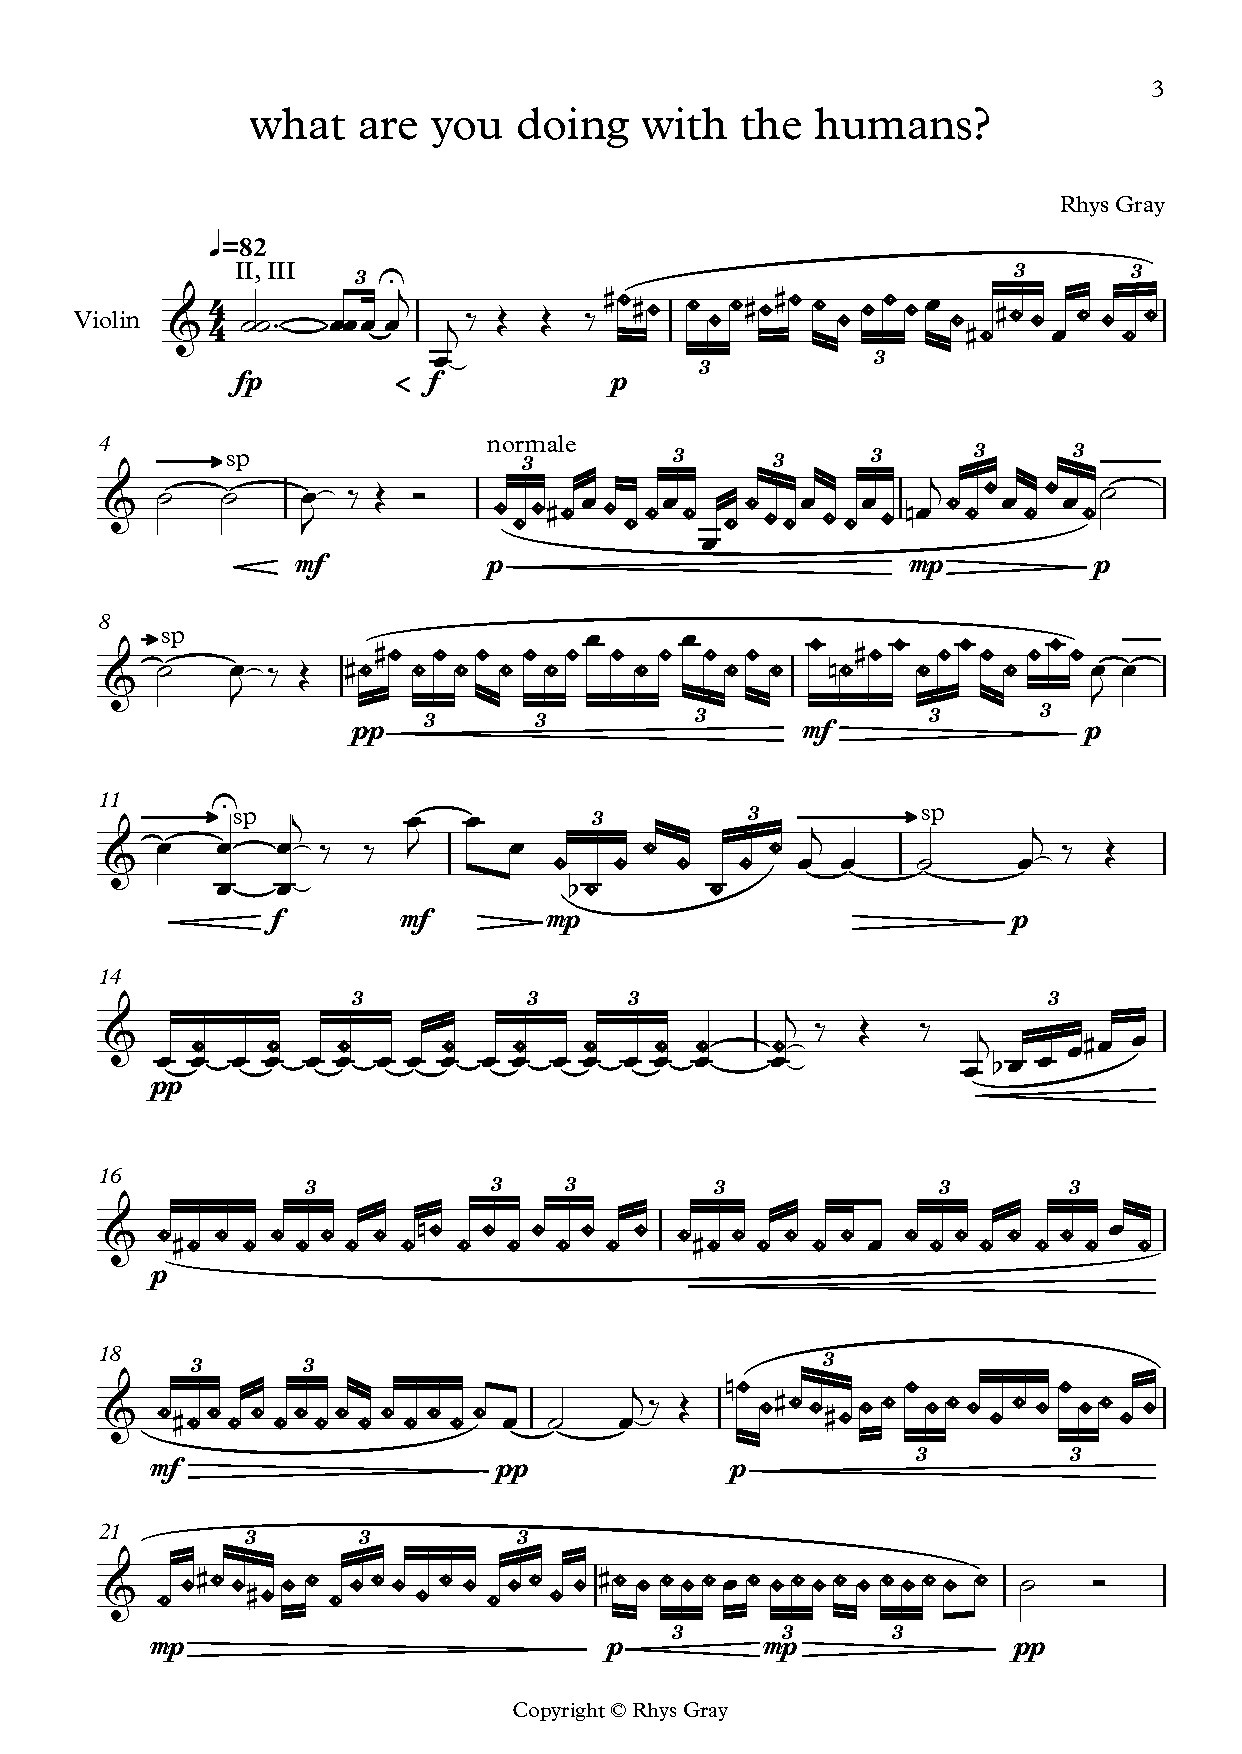
\includepdf[pages=-,pagecommand={},width=\textwidth]{resources/compositions/violin.pdf}
\label{app:The Veldt Score}
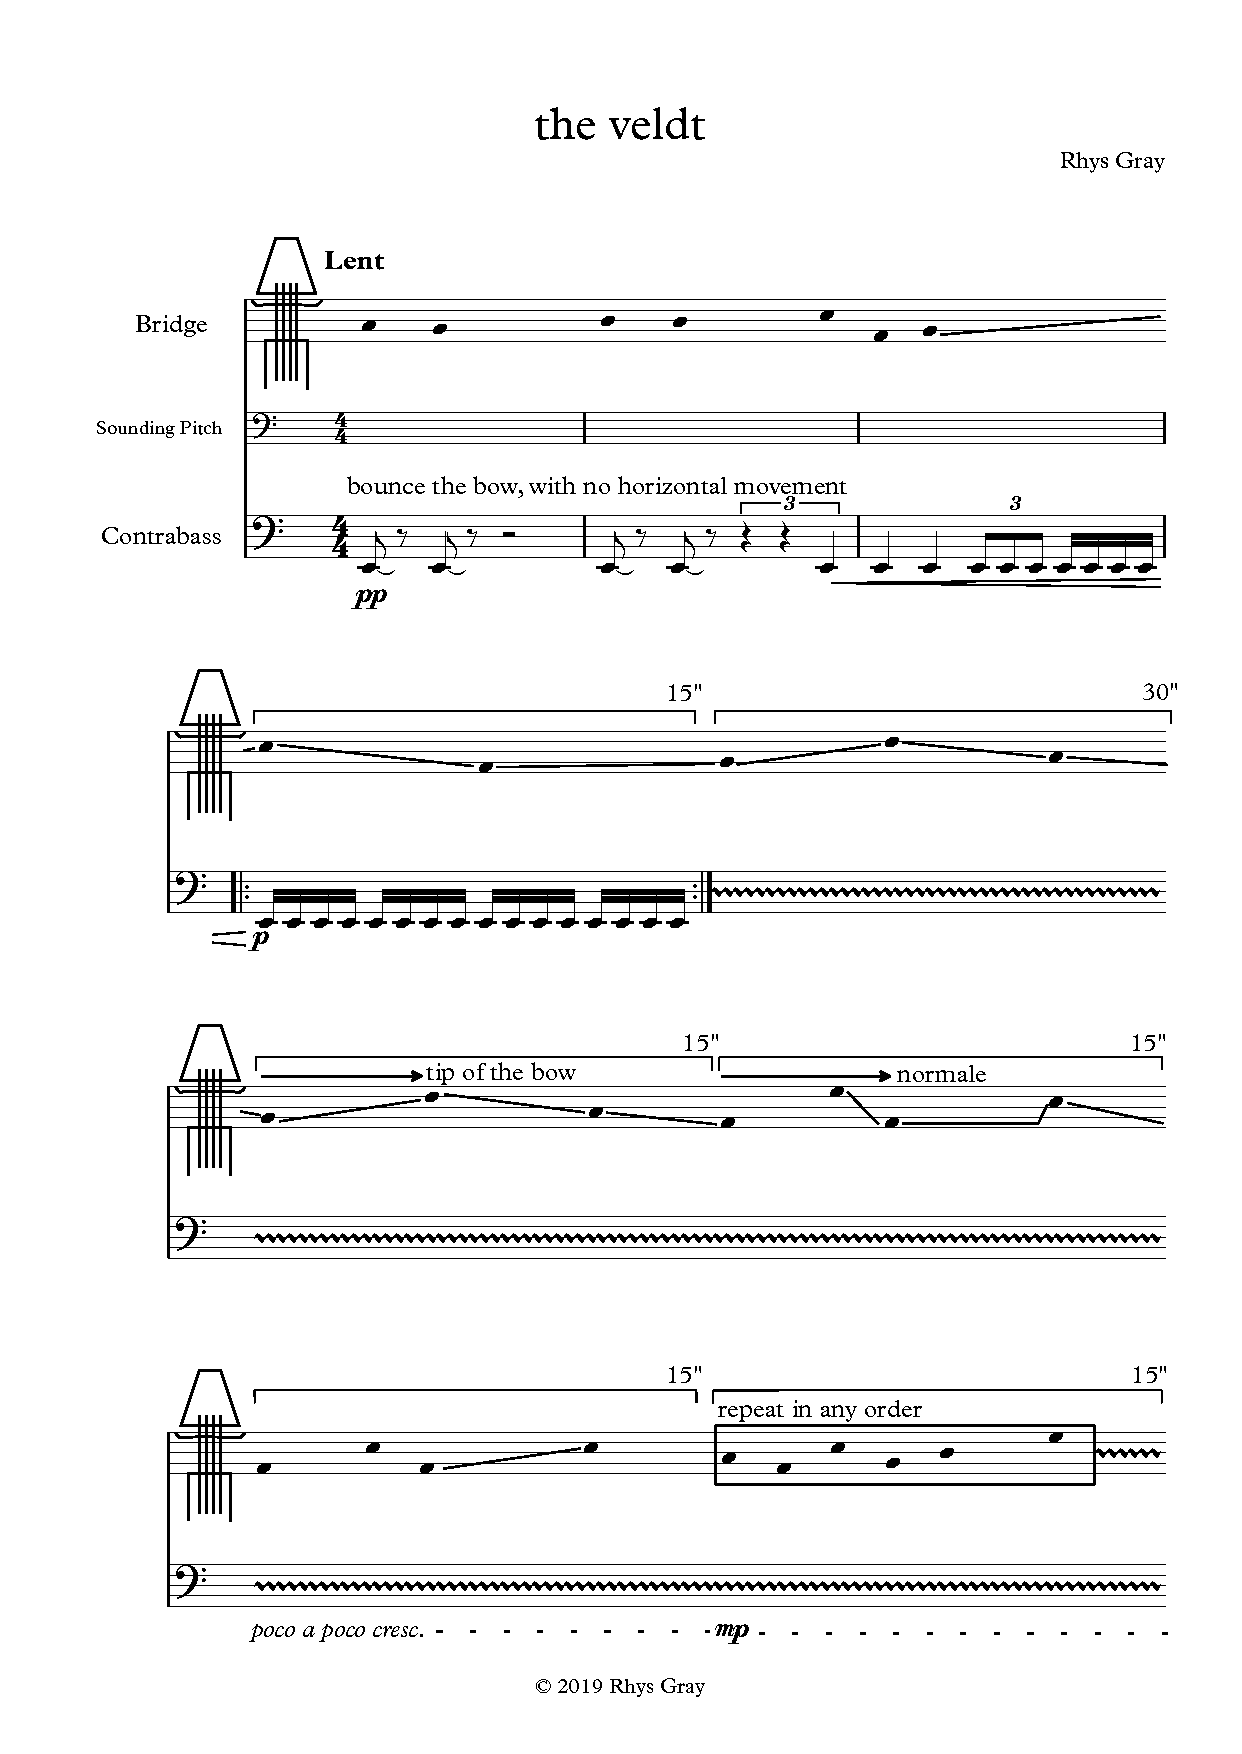
\includepdf[pages=-,pagecommand={}]{resources/compositions/bass.pdf}